\documentclass[11pt ,english,a4paper]{article}

\usepackage[english]{babel}
\usepackage[IL2]{fontenc}
\usepackage[utf8]{inputenc}
\usepackage{graphicx}
\usepackage{url}
\usepackage{hyperref}
\usepackage{times}
\usepackage{setspace}
\usepackage{float}

\setstretch{1.5}
\pagestyle{headings}

\title{Comparative Analysis of the Efficiency of Techniques for Detecting Misinformation in Healthcare Data\thanks{Semestral project in subject Engineering Methods, ac. year 2023/24, guidance: MSc. Mirwais Ahmadzai}}

\author{Alžbeta Žiarovská\\[2pt]
	{\small Slovak University of Technology in Bratislava}\\
	{\small Faculty of Informatics and Information Technologies}\\
	{\small \texttt{xziarovska@stuba.sk}}
	}

\date{\small 5th November 2023}



\begin{document}

\maketitle
\newpage

\begin{abstract}
This article offers a comparative analysis of efficiency of two machine learning techniques (Naïve Bayes and Support Vector Machine) used for information retrieval a detection of misinformation in a field of healthcare data. Article is a literature review and offers an outline of current situation of these machine learning methods. The comparison has found a negligible difference between accuracy of the two compared techniques in their efficiency for data retrieval as means of combating medical misinformation. There is a possibility of the use of my findings in everyday practice as these finding can point out that machine learning models are effective in sorting and retrieval of the medical information on the internet. 
\end{abstract}
\newpage

\section{Introduction}\label{intro}

In this article I discuss the current situation regarding spread of misinformation in the medical field and how can machine learning techniques contribute to retrieval and processing of healthcare data. This topic is very important in the aftermath of the global COVID-19 pandemic, as we have seen a great rise of various misinformation in the healthcare domain, which provide danger to public health or even lives. \cite{war18dr}. The main problem in my perception is, that the easy access to all the information on the Internet, while valuable, can increase fear and anxiety and ultimately lead to the delay of diagnosis and receiving the effective healthcare when the information is not perceived correctly \cite{wa19sys}. I will argue that various machine learning models Naïve Bayes and Support Vector Machine can be used as a potential way of data retrieval that has ability to counter prevalence of misinformation in healthcare.

\section{Related work}

The topic of misinformation is quite often researched. Many of the works I came across use information retrieval done by machine learning as a way of recognizing misinformation found in healthcare data. Some of this work is focused on comparing the different machine learning techniques \cite{sha20mach}, \cite{pod19mach}. Focus of these researches are to introduce how these methods work. Other articles bring new way information retrieval technique \cite{chap22unmask} by combining the two, or even more techniques. Plenty of research have been also done in a field of processing medical misinformation, which is a important part of my article \cite{gu20misinfo}, \cite{cook15misinfo}, \cite{wa19sys}. These articles mostly focus on defining misinformation their possible cause and consequences. By making a revision of these works, I gain deeper knowledge of the healthcare misinformation and get a better starting point to make my own analysis.

\section{Methodology}\label{methodology}

For this article my methodology is based on an in-depth literature review of articles and researches debating medical misinformation and machine learning techniques used for information retrieval to detect such misinformation. I extracted relevant data from the literature and based on them I concluded a comparative analysis of efficiency of machine learning models as a way to find the medical misinformation. The two machine learning techniques I am focusing on are Naïve Bayes and Support Vector Machine. I introduce these techniques and compare their efficiency in order to establish which one is the most suitable for retrieving healthcare misinformation and its detection. The comparison of their efficiency is done by comparing the accuracy rates of detecting and correctly categorizing false information among true information. 

\section{Misinformation in healthcare}\label{mih}

\paragraph{Difference between misinformation and disinformation}
The terms \emph{misinformation} and \emph{disinformation} are much the same, however, a small, but crucial difference can be distinguished. The difference between the two is a intention with which the false information is made accessible to the public and spread. Whilst the misinformation is usually created without direct intention of misleading and spreading false, meaning the person who put the information into the world might not actually know it is not true. On the other hand, disinformation is essentially created to spread false information. An example of such activity can be political propaganda \cite{gu20misinfo} \cite{cook15misinfo}. Even though the terms are not meaning the same, for the purpose of this article they are used as synonyms, because the author's knowledge, whether the information is factual, is negligible in the scope of its false recognition.

\paragraph{Health care misinformation}
A vast majority of people is using the Internet and social media for entertainment or information seeking. However, with the possibility of immediate communication and sharing, it has become easy to spread misinformation online \cite{wa19sys}. During the COVID-19 pandemic there have been a great amount of healthcare misinformation spread regarding vaccines and their effectiveness \cite{chap22unmask}. Internet is easily accessible and more and more people are looking for relevant health information without the proper knowledge of how to distinguish, whether the information is true. This can lead to unintentionally getting false information, as many websites do not provide accurate medical information \cite{cook15misinfo}. Another example of current situation can be the popular misinformation about vaccines causing autism, which was repeatedly proven as nonfactual information \cite{wa19sys}. 
The spread of medical misinformation is not only occurring in the 21st century. In the past there was false information about public health impact of smoking spread by tobacco companies, which was later proven as false. \cite{cook15misinfo}.

\section{Machine learning techniques} \label{tech}

\subsection{Naïve Bayes}\label{nb}
The Naïve Bayes method is a linear probabilistic machine learning technique based on Bayes theorem. This method uses probability of the events without taking their relation into the consideration \cite{sha20mach}. This approach might not look to be the best, as the words have their order and are related one to other in articles. However, the opposite is true, as the linear models are capable of achieving high efficiency despite their simplicity \cite{pod19mach}. The accuracy of Naïve Bayes (as well as other machine learning methods) is also depended from which type of measuring the importance of the words in the documents is used. For the Naïve Bayes the results vary from 84,056\% \cite{sha20mach} to 98,71\% \cite{bar21health}. These percentages represent the accuracy of distinguishing false and true information by machine. The closer analysis of these differences and their comparison is given in Section \ref{analysis}.

Formula for Naïve Bayes calculation: \cite{sha20mach}

\begin{equation}
P(A|B) = \frac{P(B|A)P(A)}{P(B)}
\end{equation}

P(A\textbar B) is the probability of event A happening supposing, that event B has already occurred.

\subsection{Support Vector Machine}\label{svm}
Support vector machine might be classified as a binary technique, as its methodology is to divide the data it was given into two categories \cite{pod19mach} (in the case of misinformation detection into true and false information). The division is made by creating a hyperplane (a object in the vector space with one dimension less than the vector space itself \cite{sha20mach})
As it was mentioned in the section \ref{nb} about Naïve Bayes, the result can vary according to the technique used for analysis of the given data and for the Support Vector Machine percentages of accuracy are on a scale from 83\% \cite{chap22unmask} to 95,05\% \cite{sha20mach}.

\section{Analysis and results}\label{analysis}
I have introduced a couple of machine learning techniques to retrieve and detect misinformation in healthcare in order to compare their effectiveness. In this section I compare their results and analyze their performance. To do so, I have searched of numeric expression of their accuracy in percentage - how big is the proportion of correctly categorized claims or documents. As mentioned in Section \ref{methodology}, this analysis is based on review of existing literature, which allows me to access finding from multiple sources. Each source provides different results which can be found in Table \ref{table:results} with corresponding superscripts of the source that the number comes from. 

\begin{table}[H]
\centering
\begin{tabular}{||c c||} 
 \hline
Naïve Bayes & Support Vector Machine\\ [0.5ex] 
 \hline\hline
 $88.37\%^{1}$ & $84\%^{1}$  \\
 \hline
 $98.71\%^{2}$ & $94.17\%^{2}$  \\
 \hline
 $85.85\%^{3}$ & $90.95\%^{3}$  \\
 \hline
 $84.06\%^{4}$ & $95.05\%^{4}$  \\ [1ex]
 \hline
\end{tabular}
\caption{\centering Accuracy of machine learning techniques in misinformation detection according to various researches, 1 - \cite{chap22unmask}, 2 - \cite{bar21health}, 3 - \cite{pod19mach}, 4 - \cite{sha20mach}}
\label{table:results}
\end{table}

According to the results of this comparison, Support Vector Machine is slightly more efficient in processing medical misinformation with average accuracy rate of 91.04\%. However, the Naïve Bayes method is behind just by a little bit with the average percentage of 89.25\%. The average accuracy rate of information retrieval using Naïve Bayes or Support Vector Machine can be seen in Figure \ref{f:average}. These result are not so greatly differing from each other and it shows, that machine learning techniques nowadays are highly advanced and can achieve significant results.

\begin{figure}[H]
\centering
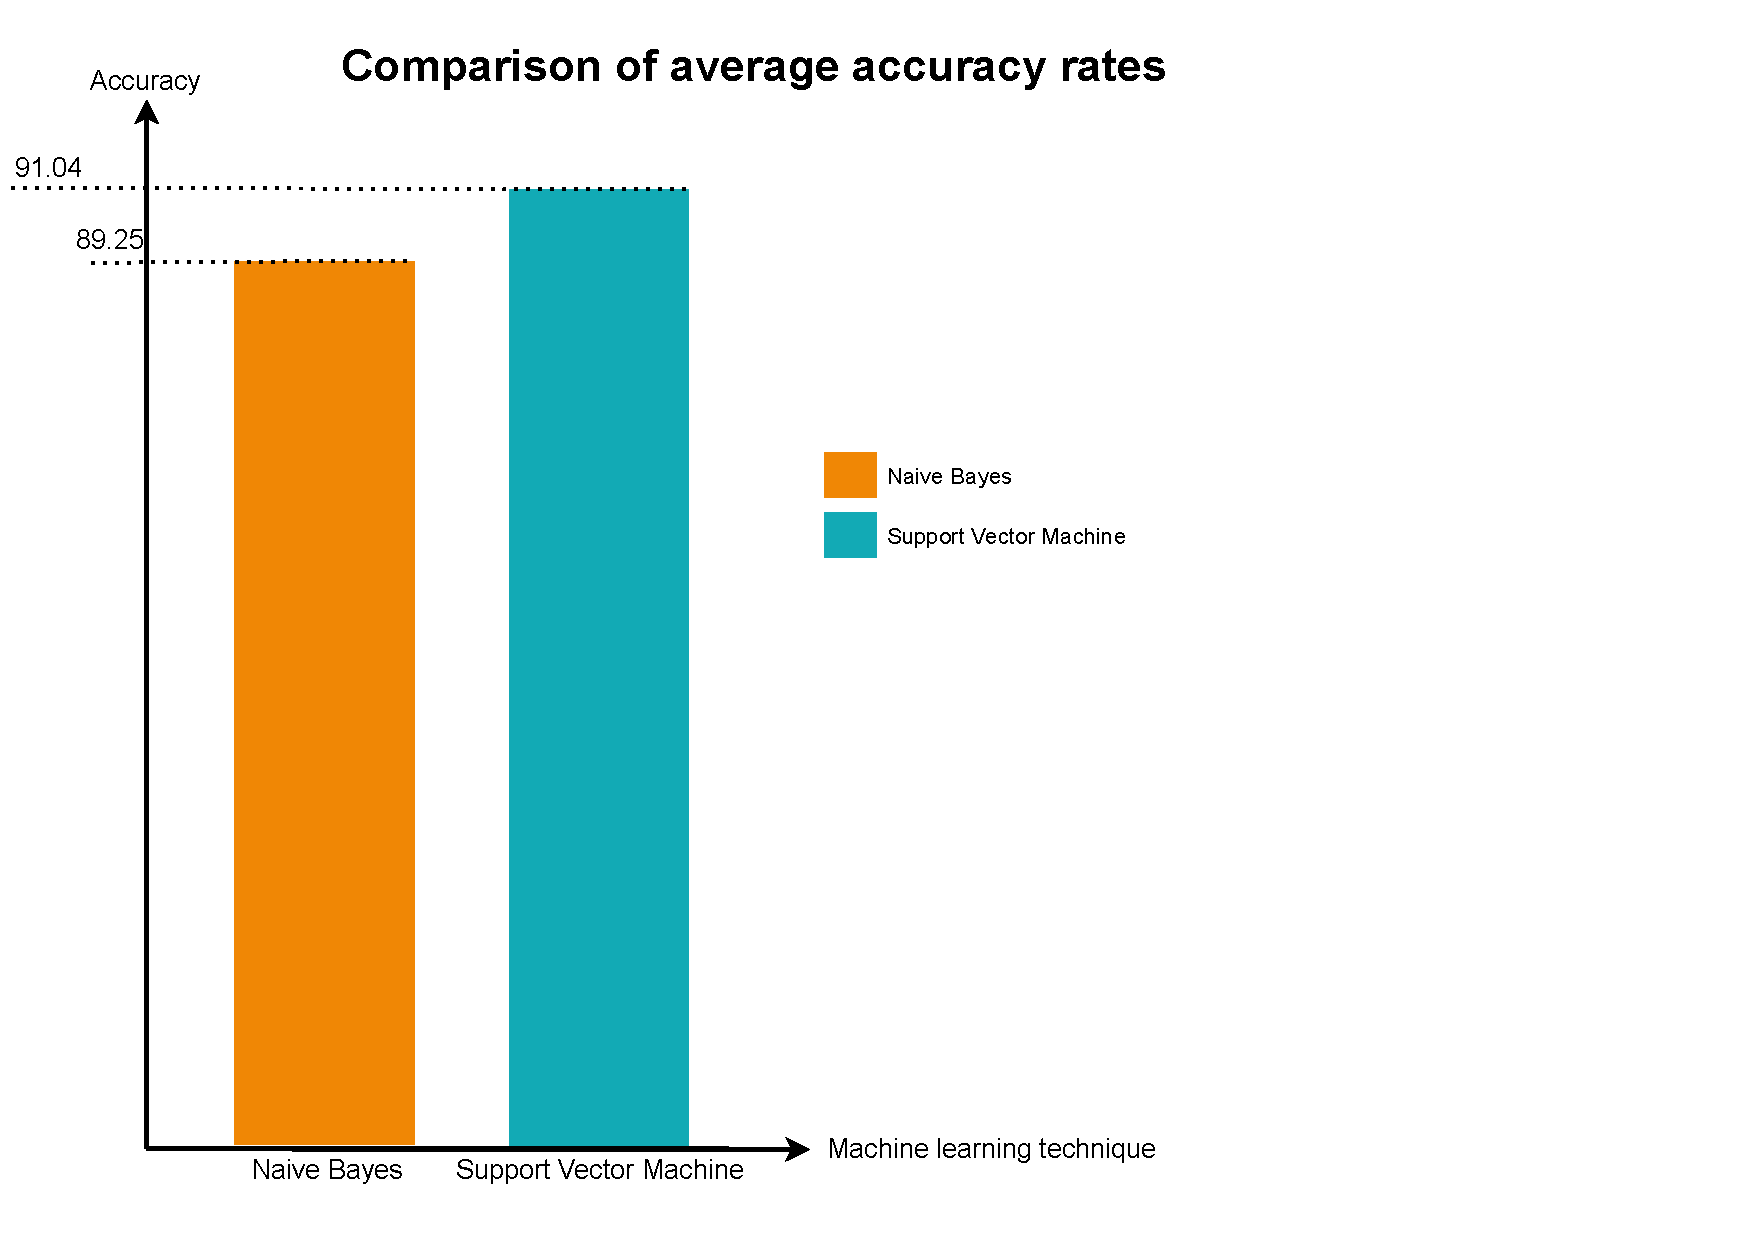
\includegraphics[scale=0.4]{average_accuracy.pdf}
\caption{\centering Comparison of average accuracy.}
\label{f:average}
\end{figure}

\section{Discussion}

I have found several evidence to confirm, that machine learning techniques can be a very useful (and accurate) tool in retrieving and recognizing misinformation in healthcare with both Naïve Bayes and Support Vector Machine showing satisfactory performance. In my article I used accuracy rate results of these two machine learning techniques used for misinformation detection to compare their efficiency. The Support Vector Machine is according to the result more accurate, however the difference is trivial. It is important to acknowledge, that my article is based on literature review of existing researches, which creates limitations by the range of the researches used for the purpose of this article.

\section{Conclusion}\label{conclusion}

This article is an in-depth literature review of articles researching misinformation retrieval and detection in healthcare data using machine learning methods. I have compared results from several resources and based on these I have created an analysis of two machine learning techniques I focused on. In order to provide analysis of their efficiency I came to conclusion, that the machine learning techniques are highly advanced and can efficiently differentiate between factual and nonfactual information. This can provide solution to the main problem I mentioned in the beginning of the article - people possibly not perceiving the information found on the Internet correctly. With the use of machine learning techniques there is a possibility of decreasing spread of medical misinformation by having effective tool for information processing.

\newpage
\bibliography{127323_bibliography}
\bibliographystyle{plain}
\end{document}
